
\usetikzlibrary{shadows}
\usetikzlibrary{automata, positioning, arrows, calc}
      \definecolor{falured}{rgb}{0.5, 0.09, 0.09}
     \newcommand{\fmbtsymbex}[1]{\textcolor{falured}{ #1}}
     \newcommand{\fmbtsymbexReg}[1]{ \textcolor{falured}{ #1} }
     \definecolor{mycolorData}{rgb}{0.07, 0.04, 0.56}


      \definecolor{mycolorF}{rgb}{0.973, 0.882, 0.882} 
     \definecolor{mycolorP}{rgb}{0.902, 0.957, 0.918}
     \definecolor{mycolorI}{rgb}{1.000, 0.969, 0.800}


\tikzset{
	%->,  % makes the edges directed
	%>=stealth, 
	% makes the arrow heads bold
	shorten >=2pt, shorten <=2pt, % shorten the arrow
	node distance=3cm, % specifies the minimum distance between two nodes. Change if n
	every state/.style={draw=blue!55,very thick,fill=blue!20}, % sets the properties for each ’state’ n
	initial text=$ $, % sets the text that appears on the start arrow
	%node distance=2.5cm,
    %every edge/.style={draw, bend left=20, ->}
    circled node/.style={rectangle,draw, inner sep=0, minimum size=1.5em},
    better circled node/.style={circled node,text height=.8em,text depth=.25em},
    }
\renewcommand{\arraystretch}{0.9}

%\newcommand{\myhash}{\raisebox{\depth}{\scalebox{0.8}{\#}}}
\newcommand{\myhash}{\raisebox{\depth}{\scalebox{0.8}{\#}}} 
\newcommand{\mydollar}{\raisebox{\depth}{\scalebox{0.8}{\$}}} 

	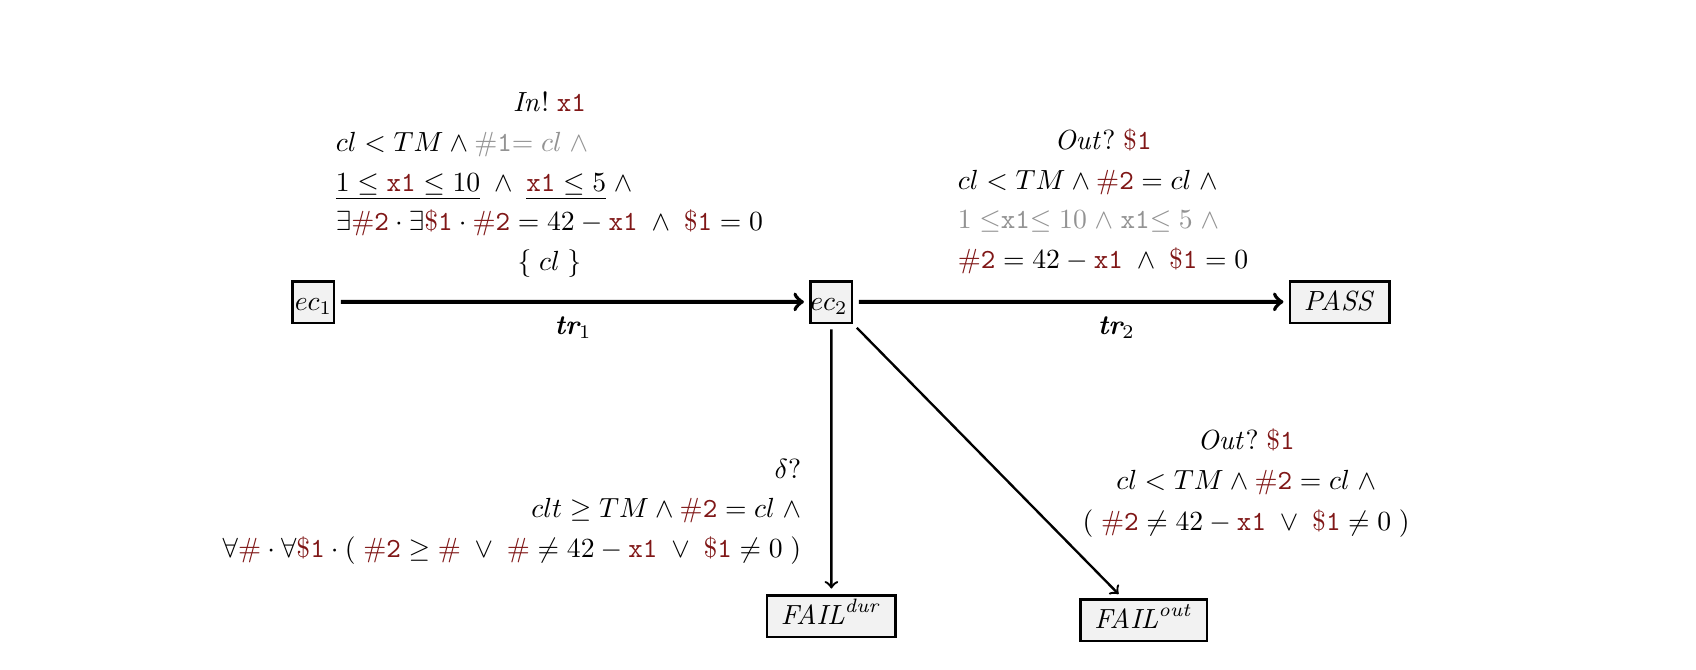
\begin{tikzpicture}
    [xscale=1.75, yscale=1.75%,font=\small %footnotesize
    ] 
	%\draw[fill=gray!20, draw=none]  (2,21.1) rectangle (10.1,15);
%\draw[fill=gray!20, draw=none]  (10.1,11.7) rectangle (-3.3,15.6);

%	\coordinate (v17) at (3,20.7) {} {};
% \draw[line width=0.3mm,draw=mycolorData,drop shadow={fill=mycolorData},fill=white] (v17) 
%     -- (11,20.7)
%     -- (11,12.328)
%     -- (-3.4,12.328)
%     -- (-3.4,15.8)
%     -- (3,15.8)
%     -- cycle;

\draw[line width=0.3mm,draw=none,fill=white]  (-2.1,12.3) 
rectangle (9.8,8.276);


% \draw[draw=mycolorP, line width=1.5mm]  (0.04,18.608) -- (0.04,17.0328);
% \draw[draw=mycolorP, line width=1.5mm, bend left=20]   (-0.104,16.9328)edge (-0.152,18.6094) ;
% \draw[draw=mycolorP, line width=1.5mm,dotted] (3.6,19.3029) -- (3.6,18.82);
% \draw[draw=mycolorP, line width=1.5mm,dotted] (-0.804,19.047) -- (-0.304,19.047);
% \draw[draw=mycolorP, line width=1.5mm] (3.6,18.116) -- (3.6,16.424);
% \draw[draw=mycolorP, line width=1.5mm] (3.312,15.8734) -- (0.74,14.651);
% \draw[draw=mycolorP, line width=1.5mm] (-0.168,10.3144) -- (3.276,10.3144);
% \draw[draw=mycolorP, line width=1.5mm] (4.076,10.3144) -- (7.288,10.3144);


	

%%%%%%%%%%%%%%%%%%%%%%%%%%%%
%%%%%%%%%%%%% TEST CASE%%%%%%%%%
%%%%%%%%%%%%%%%%%%%%%%%
%%%%%%%%%%%%%%%%%%%%%%%%%%%%%%%

\node[circled node,line width=.3mm,fill=gray!10] (v1) at (-0.0264,10.308) {$\!\!\!\!
\begin{array}{c}
ec_1 
\end{array}\!\!\!\!
$};

	

	
		

	

\node[circled node,line width=.3mm,fill=gray!10] (v2) at (3.732,10.308) {$\!\!\!\!
\begin{array}{c}
ec_2 
\end{array}\!\!\!
$};

	
	


	
	

\node[circled node,line width=.3mm,fill=gray!10] (v3) at (7.4212,10.308) {$%\!\!\!\!
\begin{array}{c}
\mathit{\text{PASS}}
\end{array}%\!\!\!\!
$};

\node[circled node,line width=.3mm,fill=gray!10] (v4) at (6,8) {$%\!\!\!\!
\begin{array}{c}

\mathit{\text{FAIL}}^{\mathit{out}}
\end{array}%\!\!\!\!
$};



\node[circled node,line width=.3mm,fill=gray!10] (v5) at (3.732,8.0286) {$%\!\!\!\!
\begin{array}{c}

\mathit{\text{FAIL}}^{\mathit{dur}}
\end{array}%\!\!\!\!
$};












%\draw[dotted]  (v1) edge (v5);





\node at (5.704,11.0416) {$
 \def\arraystretch{1.2} 
\begin{array}{c}
\mathit{Out}?\; \fmbtsymbex{\mathtt{\$1}}
\\
%\left[
%\left[
\begin{array}{l}
cl < \text{TM} \land \fmbtsymbex{\mathtt{\#2}} = cl  \;\land
\\

\textcolor{gray!85}{1 \le} \fmbtsymbexReg{\textcolor{gray!85}{\mathtt{x1}}} \textcolor{gray!85}{\le 10 \;\land\;}
 \fmbtsymbexReg{\textcolor{gray!85}{\mathtt{x1}}} \textcolor{gray!85}{\le 5 \;\land\; } \\ \fmbtsymbex{\mathtt{\#2}}=42-\fmbtsymbexReg{\mathtt{x1}} \;\land\;
 \fmbtsymbex{\mathtt{\$1}}=0 

\end{array}
%\right]
\end{array}
$};


\node at (6.7426,9) {$
 \def\arraystretch{1.2} 
\begin{array}{c}
\mathit{Out}?\; \fmbtsymbex{\mathtt{\$1}}
\\%[1ex]
%\left[
%\left[
\begin{array}{c}
cl < \text{TM} \land \fmbtsymbex{\mathtt{\#2}} = cl  \;\land
\\
\begin{array}{l}

(\;\fmbtsymbex{\mathtt{\#2}}\neq 42-\fmbtsymbexReg{\mathtt{x1}} \;\lor\; 
\fmbtsymbex{\mathtt{\$1}}\neq 0 \;)
 \end{array}
\end{array}
%\right]
%\right]
\end{array}
$};


\node at (1.6864,11.1716) {$
 \def\arraystretch{1.2} 
\begin{array}{c}
\mathit{In}!\; \fmbtsymbexReg{\mathtt{x1}} 
\\
%\left[
%\left[ 

\begin{array}{l}
cl < \text{TM} \land 
\fmbtsymbex{\textcolor{gray!85}{\mathtt{\#1}}} \textcolor{gray!85}{= cl  \;\land}
\\
\underline{1 \le \fmbtsymbexReg{\mathtt{x1}} \le 10} \;\land\;   \underline{\fmbtsymbexReg{\mathtt{x1}} \le 5  } \;\land
\\
 \exists \fmbtsymbex{\mathtt{\#2}} \cdot
 \exists  \fmbtsymbex{\mathtt{\$1}}
\cdot 
\fmbtsymbex{\mathtt{\#2}}=42-\fmbtsymbexReg{\mathtt{x1}} \;\land \;\fmbtsymbex{\mathtt{\$1}}=0  
\end{array}
%\right]
%\right]
\\
\{\; cl \;\}
\end{array}
$};



	

\node at (1.4142,8.7998) {$
 \def\arraystretch{1.2} 
\begin{array}{r}
\delta?
\\
clt \ge \text{TM} \land \fmbtsymbex{\mathtt{\#2}} = cl  \;\land
\\
\forall \fmbtsymbex{ \mathtt{\#}} \cdot \forall \fmbtsymbex{ \mathtt{\$1}} \cdot(\;
\fmbtsymbex{\mathtt{\#2}} \geq \fmbtsymbex{\mathtt{\#}}  
\;\lor\;\fmbtsymbex{\mathtt{\#}}\neq 42-\fmbtsymbexReg{\mathtt{x1}}  \;\lor\; 
\fmbtsymbex{\mathtt{\$1}}\neq 0\;)
\end{array}
$};






	\node at (1.8576,10.124) {$\textbf{\em tr}_1$};
\node at (5.8,10.124) {$\textbf{\em tr}_2$};






\draw
[ line width=.5mm , -> ]
(v1) edge (v2);
\draw
[ line width=.5mm , -> ]
(v2) edge (v3);





\draw 
[ line width=.3mm , -> ]
(v2) edge (v4);



\draw  
[ line width=.3mm , -> ]
(v2) edge (v5);





    


\end{tikzpicture}